% =============================================================
% Chapter 4: Plan Of Project
% =============================================================

\newpage
\vspace*{\fill}
\begin{center}
\textbf{\Huge{Chapter 4}}\\
\vspace{5mm}
\textbf{\Huge{Plan Of Project}}
\end{center}
\vspace*{\fill}
\newpage

\titleformat{\chapter}[block]{\normalfont}{}{0pt}{}
\titlespacing{\chapter}{0pt}{-2em}{0pt}
\chapter[Plan Of Project]{}
\thispagestyle{fancy}
\titleformat{\chapter}[display]{\vspace{1cm}\normalfont\Large\bfseries\centering}{\chaptertitlename\ \thechapter}{20pt}{\vspace{0pt}}
\titlespacing*{\chapter}{0pt}{-50pt}{20pt}

\section{Methodology}
\justify

AyurSpace uses a highly decoupled method that combines artificial intelligence, mobile frontend engineering, and backend cloud infrastructure.

\item[$\bullet$]\textbf{ Presentation Layer (Flutter) :}\\ Built entirely in Flutter, responsible for UI rendering, capturing user input, translating languages (ARB files), and displaying state updates effectively across Android and iOS platforms.

\item[$\bullet$]\textbf{ State Management :}\\ We utilize Riverpod for reactive state management and dependency injection. Riverpod isolates UI from internal business logic, enabling components to listen to streams for live changes (e.g., chat message history, dosha quiz progression).

\item[$\bullet$]\textbf{ Domain Layer (Core Business Logic) :}\\ Contains pure Dart classes mapping Ayurvedic concepts into technical objects---like \texttt{Plant}, \texttt{Dosha}, and \texttt{Remedy}.

\item[$\bullet$]\textbf{ Plant Taxonomy Integration (Plant.id API) :  }\\When a user scans a plant, the photo is compressed locally and sent to the Plant.id residual network, acting as a taxonomic classifier identifying the technical species name.

\item[$\bullet$]\textbf{ LLM Contextualizing (Gemini API) : }\\ After technical identification, a prompt is generated for Google Gemini API, employing Chain-of-Thought (CoT) prompting techniques. Gemini receives the Latin name to synthesize Ayurvedic properties such as Rasa, Guna, Virya, and home remedies.

\item[$\bullet$]\textbf{ Cloud Storage and Auth :   }\\To ensure accurate user profiling across devices, we employ Firebase Authentication and Cloud Firestore. It powers live synchronization of users' scanning history, determined dosha conditions, and profile data securely.


\newpage
\section{Project Plan (Timeline Diagram)}
A Gantt chart illustrates the timeline of various project modules from Planning to Deployment.

\renewcommand{\thefigure}{4.1}
\renewcommand{\figurename}{Figure}
\begin{figure}[!htbp]
\begin{center}
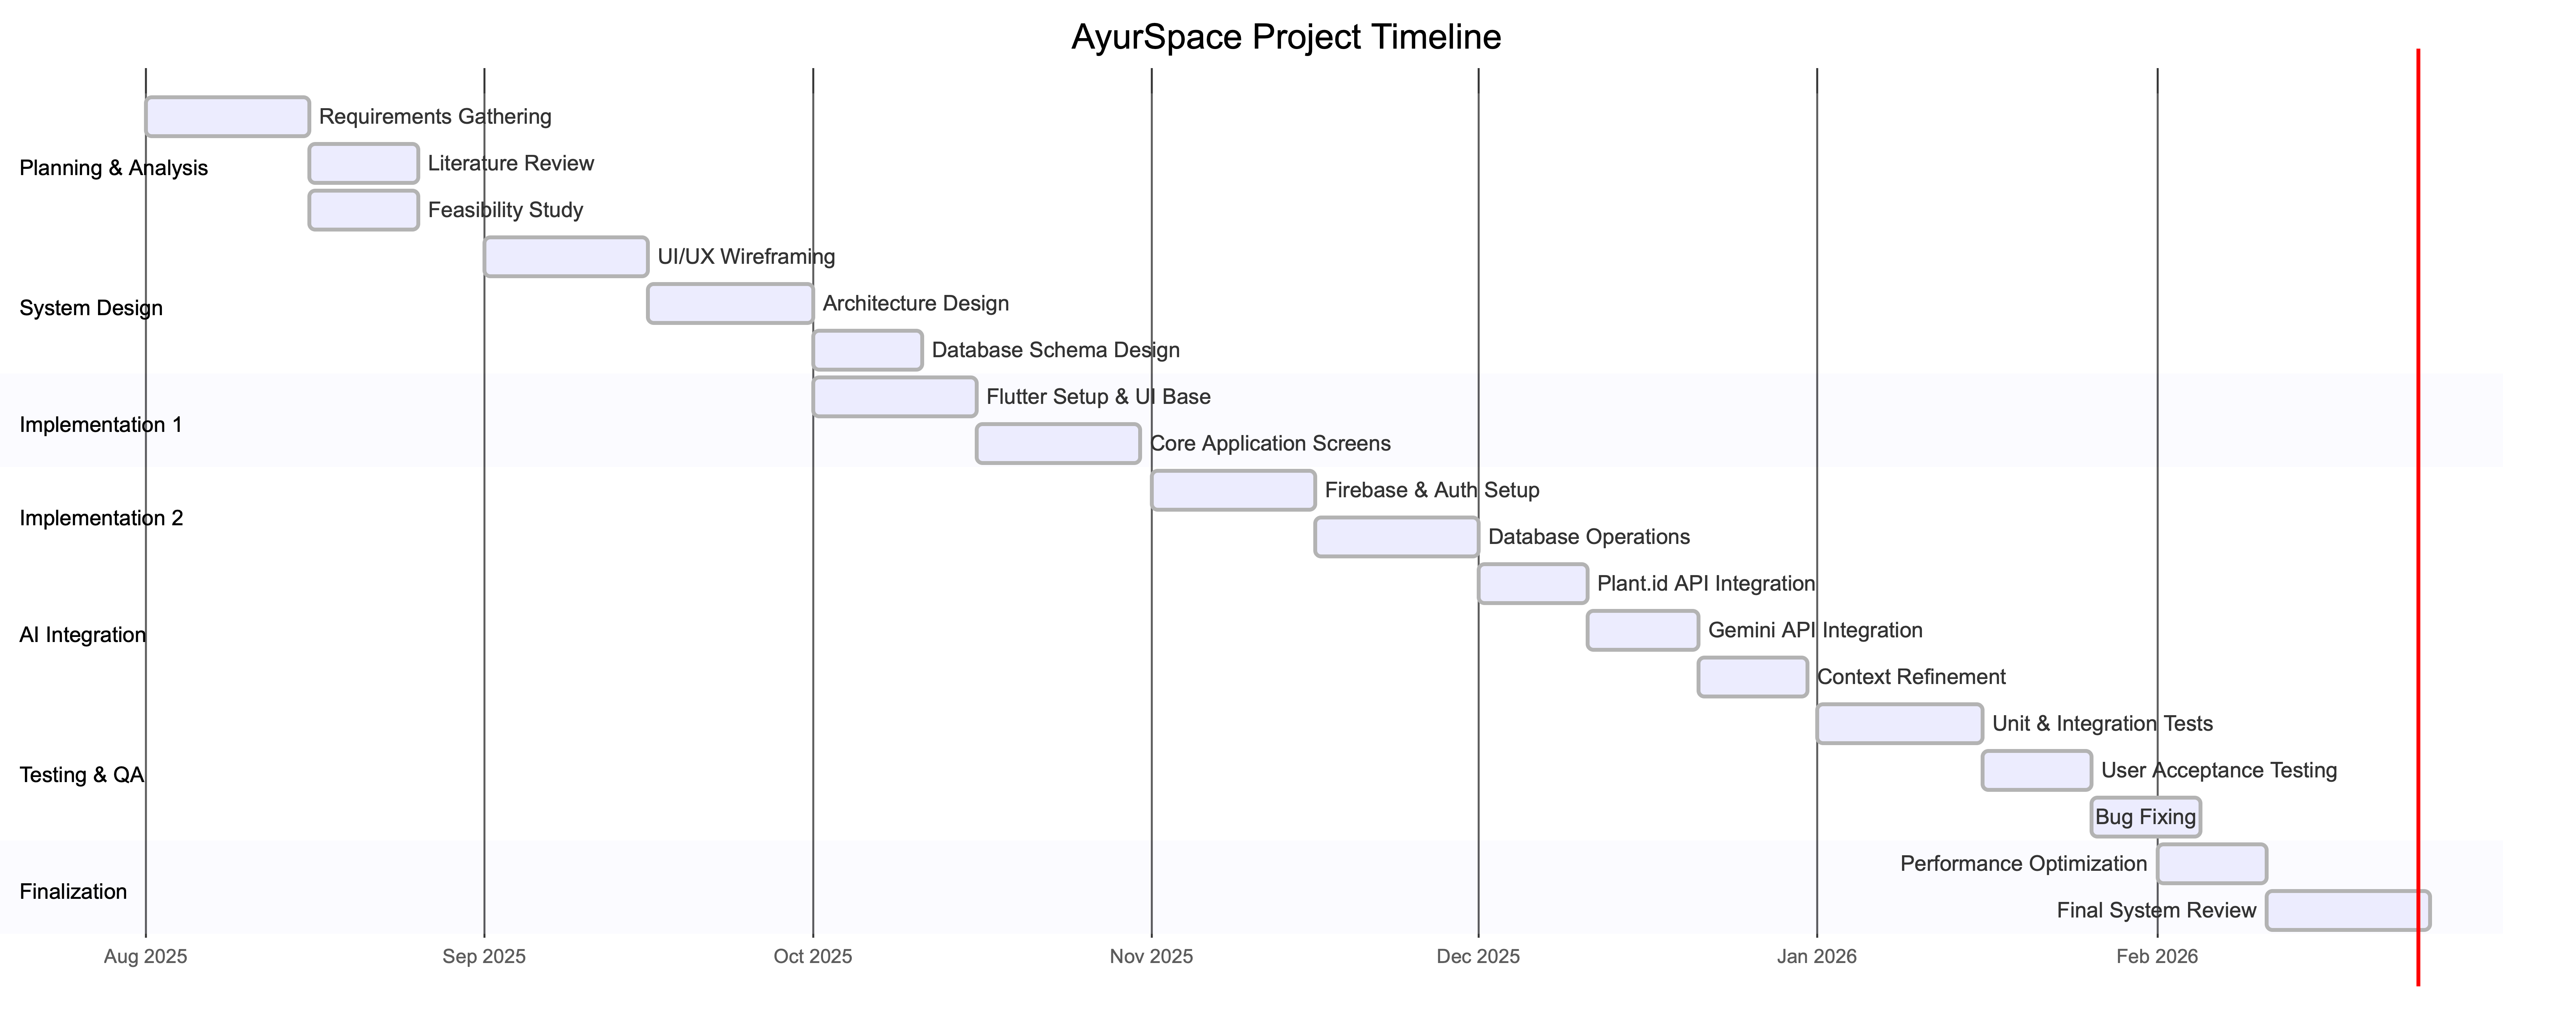
\includegraphics[width=\textwidth,height=0.4\textheight,keepaspectratio]{placeholder_gantt.png}
\caption{Project Plan Timeline}
\end{center}
\end{figure}
The timeline ensures efficient project management, tracking module initiation and deadlines for the UI layout, API integration, testing, and deployment.

\newpage
\section{Proposed System Architecture}
\justify
The AyurSpace system architecture is built as a cloud-native mobile application that follows Clean Architecture principles. The system works on a Client-Server model, where the Flutter mobile client is the orchestration engine that links different microservices. The application logic is highly decoupled from the presentation layer, relying on dependency injection and robust state management.

\subsection{Layered Architecture}
The software consists of three primary layers:
\begin{enumerate}
    \item \textbf{Presentation Layer}: Built entirely in Flutter. Responsible for UI rendering, capturing user input, and displaying state updates.
    \item \textbf{Domain Layer}: Contains the core business logic, entities, and use-case definitions. Functions independently of any specific data source or UI framework.
    \item \textbf{Data Layer}: Handles the retrieval and storage of data from local caches, Firebase, and third-party APIs like Plant.id and Google Gemini.
\end{enumerate}

\subsection{Directory Structure}
The repository structure enforces this separation of concerns:
\begin{lstlisting}[language=bash]
lib/
|-- config/          # Global configs (API keys, theme, router)
|-- data/            # Models, Repositories, Data Sources
|   |-- models/
|   |-- repositories/
|   |-- sources/
|-- providers/       # Riverpod Providers and Notifiers
|-- screens/         # UI Screens
|-- services/        # Service wrappers (API clients, Firebase setup)
|-- utils/           # Utilities and helpers
|-- widgets/         # Reusable UI components
\end{lstlisting}

\subsection{Hybrid Neuro-Symbolic Inference Pipeline}
The system's intelligence relies on a two-step hybrid approach:
\begin{itemize}
    \item \textbf{Discriminative Phase (Vision)}: An image uploaded by the user is compressed and sent to the Plant.id API. The API uses a Convolutional Neural Network (CNN) to return the scientific classification (Taxonomy) with a confidence score.
    \item \textbf{Generative Phase (Language)}: The scientific name identified by the CNN is passed as a prompt to the Google Gemini Large Language Model (LLM). Gemini is constrained via strict system prompts to act as an Ayurvedic expert, returning the \textit{Dosha} properties, uses, and precautions associated with the plant.
\end{itemize}

\renewcommand{\thefigure}{4.2}
\begin{figure}[!htbp]
\begin{mdframed}
    \centering
    
\includegraphics[width=0.7\linewidth,keepaspectratio]{placeholder_system_arch.png}
\end{mdframed}
\caption{Proposed System Architecture}
\end{figure}
